\section{Design of the sound scene DSL}
\label{sec:design-sound-spec}

From the overall design decisions for the entire sound system and game
system, some parts of the design of the sound scene DSL subsystem were
given automatically: we have to interact with a \texttt{Redis} database, with
an \texttt{AMQP} communication system, and send JSON packages according to a
fixed format in order to control the lower level system.

On top of this, we had requirements for swift development, for ease of
use, and for minimizing the amount of extra parsers to write. These
criteria were central in selecting Haskell as a platform for the tool:
out of the platforms that members of the workgroup were familiar with,
Haskell was far more capable of quick development and quick automatic
generation of parsers and serializers than all the alternatives. 

Our system ended up depending on a family of Haskell packages that
cover many of the interoperability requirements. In total, we relied
on 
\texttt{aeson}\cite{aeson}, 
\texttt{amqp}\cite{amqp}, 
\texttt{attoparsec}\cite{attoparsec}, 
\texttt{base}\cite{haskell}, 
\texttt{bytestring}\cite{bytestring}, \\
\texttt{containers}\cite{containers}, 
\texttt{ghc-prim}\cite{haskell}, 
\texttt{hedis}\cite{hedis}, \\
\texttt{mtl}\cite{mtl}, 
\texttt{regex-posix}\cite{regex-posix}, 
\texttt{text}\cite{text}, and\\
\texttt{unordered-containers}\cite{unordered-containers}, 
for all our library needs.

From these preconditions, we decided that the best way to construct a
DSL would be to encode all the information we would need access to in
terms of specific Haskell datatypes, so that Haskell methods for
generating parsers and serializers could be used. We combined this
recognition with the need for a hierarchy of types bridging the gap
from the human-readable game master facing DSL and the machine facing
already defined JSON protocol.

The resulting hierarchy of datatypes that we decided on was:\nopagebreak

\begin{figure}[H]
  \centering
  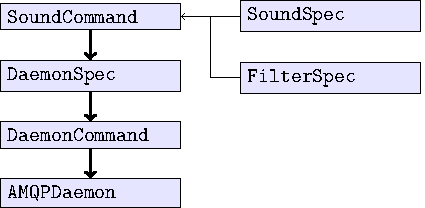
\includegraphics{figure}
  
  \caption{Dependency and compilation path hierarchy for the sound system.}
\label{fig:sshierarchy}
\end{figure}
where we have separate compilation steps to transform a \texttt{SoundCommand}
into a \texttt{DaemonSpec}, a \texttt{DaemonSpec} into a \texttt{DaemonCommand} and a
\texttt{DaemonCommand} into an \texttt{AMQPDaemon}.

These types all have different roles:
\begin{description}
\item[\tt SoundCommand] encodes all orders the system expects from
  game masters and sound designers. In order to easier design
  datatypes, we separate out the descriptions of a sound scene and of
  a reaction trigger from the command type into the subordinate types
  \texttt{SoundSpec} and \texttt{FilterSpec}.
\item[\tt DaemonSpec] encodes, abstractly, the order types the lower
  level system accepts.
\item[\tt DaemonCommand] encodes in full detail a single order for the
  lower level system.
\item[\tt AMQPDaemon] is a datatype explicitly constructed to serialize
  through \texttt{Aeson} into a JSON package that the lower level
  system can parse.
\end{description}

Here, the \texttt{SoundCommand} type encodes all orders that the game
masters and sound designers want to be able to give to the system,
\texttt{DaemonSpec} abstractly encodes all command types the lower
level system accepts, 

All datatypes derive \texttt{Read}, \texttt{Show} and \texttt{Generic}
which allows us to automate parsing both from a Read--Evaluate--Print--Loop as well as
create automatic JSON parsers and encoders from \texttt{Aeson}. 

\subsection{SoundCommand}
\label{sec:soundspec}

Our separation of the sound scene description from the Haskell layer
control commands and the automated reactive triggers builds on their
separation into different datatypes. At the top abstraction
level, there is the data type \texttt{SoundCommand} enumerating the
various commands that can be given to the system. 

\begin{verbatim}
data SoundCommand = 
    Define Id SoundSpec |
    Commit | 
    Restore | 
    Diagnostic |
    ReadState |
    ReadSounds | 
    Compile SoundSpec |
    ReadOut SoundSpec | 
    Execute Id SoundSpec |
    Trigger Id FilterSpec SoundCommand |
    SoundCommand :++ SoundCommand |
    Declare Id SoundCommand |
    Call Id | 
    Delete Id | 
    Nop
    deriving (Eq, Show, Read, Generic)
\end{verbatim}

We find commands for interacting with the database state storage:
\texttt{Commit} and \texttt{Restore}; commands for debugging and
analyzing what a particular sound scene description is interpreted to:
\texttt{Diagnostic}, \texttt{ReadState}, \texttt{ReadOut}; commands
for naming and recalling both sound scenes and entire commands:
\texttt{Define}, \texttt{Declare}, \texttt{Execute}, \texttt{Call},
\texttt{Delete}; and commands for triggering sound scenes either
through events by \texttt{Trigger} or through direct command by
\texttt{Execute}. Finally, there is \texttt{ReadSounds} that reports
available sound scenes up to a top level UI layer, and
\texttt{:++} for chaining commands together as well as a \texttt{Nop}
that can finish an automatically generated chain of commands for
programmatic creation of triggers and action chains. 

The definition uses the two types \texttt{SoundSpec} and
\texttt{FilterSpec} to parametrize its entries. These are given by

\begin{verbatim}
data SoundSpec = 
    Play File Segment Time Loudness |
    Loop File Segment Time Loudness |
    RadialDecay File Segment Time Loudness | 
    SoundSpec :+ SoundSpec | 
    Use Id |
    Stop Int Time |
    Fade Int Time Time Loudness |
    StopId Id Time |
    FadeId Id Time Time Loudness |
    NopS
    deriving (Eq, Show, Read, Generic)
\end{verbatim}
and
\begin{verbatim}
data FilterSpec = 
    FilterSpec :& FilterSpec |
    FilterSpec :| FilterSpec |
    MatchAll [FilterSpec] |
    MatchAny [FilterSpec] |
    MatchEvent String |
    MatchSender String |
    MatchKeyValue String String
    deriving (Eq, Show, Read, Generic, Ord)
\end{verbatim}

The sound scene specification fundamentally allows for playing a sound
by name or by index, either once or on an infinite loop, and for
stopping and changing volume. These are the operations understood by
the low level system as well.

In addition to these, the Haskell layer automatically generates
packages to smoothly fade between volume settings, for a spatially
distributed decaying sound scape, and for saving and recalling sound
scenes. After first attempts to design the fades, we ended up building
in support for remembering the last set volume for a sound so that
fades are given by target loudness rather than by start and stop
loudness settings.

The inclusion of \texttt{Nop} and \texttt{NopS} helps us automate
generation of lists of actions; together with the concatenation
constructions given by \texttt{:++} and \texttt{:+} there is a full
monoidal structure on both these datatypes, enabling easy generation
of composite commands from lists of command parameters. 

Since the entire system actively listens to the \texttt{AMQP} traffic of the
entire game system, it was easy to include a reactive component: using
a regular expressions-based simplistic recognition engine we were able
to write simple rules that would when matched trigger arbitrary
pre-constructed \texttt{SoundCommand} actions. The rules are encoded
using the type \texttt{FilterSpec} and their corresponding actions are
encoded with the \texttt{Trigger} constructor of
\texttt{SoundCommand}. All \texttt{AMQP} messages in the game system contain a
sender, an event key and some collection of key--value pairs all of
which can be regular expression matched with the rules specified as
\texttt{FilterSpec} entities.

\subsection{DaemonSpec}
\label{sec:daemonspec}

The \texttt{DaemonSpec} type encodes the abstract payload of a single
instruction to the low-level system. An element of type
\texttt{DaemonSpec} encodes all the descriptive information needed for
a low-level system command, without containing transient information
required for emitting any particular command package. In particular,
there is a serial ID number assigned to low-level command packages to
allow later commands to modify a running sound. These ID numbers are
not added in the \texttt{DaemonSpec} representation, but rather in the
next lower representation.

\begin{verbatim}
data DaemonSpec = 
    DaemonPlay Int Segment Time Loudness |
    DaemonLoop Int Segment Time Loudness |
    DaemonStop Int Time |
    DaemonSet Int Time Loudness 
              deriving (Eq, Show)
\end{verbatim}

\subsection{DaemonCommand}
\label{sec:daemoncommand}

The \texttt{DaemonCommand} encodes a package ready to send out to the
lower-level system. In particular, the command encodes a sequential
id-number used for later modifications of looping sounds, and sets up
a datatype for easy parsing for the receiving system.

\begin{verbatim}
data DaemonCommand = DaemonCommand {
      node :: Int,
      dcid :: Int,
      sound :: Int,
      time :: Int,
      volume_left :: Float,
      volume_right :: Float,
      command :: Int
    } deriving (Eq, Show, Generic)
\end{verbatim}

\subsection{AMQPDaemon}
\label{sec:amqpdaemon}

The type \texttt{AMQPDaemon} really only exists in order to wrap a
\texttt{DaemonCommand} item for serialization with \texttt{Aeson} and
transport in an \texttt{AMQP} package. The type is defined as:
\begin{verbatim}
data AMQPDaemon = AMQPDaemon {
      devent :: String,
      dsender :: String,
      dcmd :: DaemonCommand
    } deriving (Eq, Show, Generic)
\end{verbatim}
with custom JSON instances created by
\begin{verbatim}
instance FromJSON AMQPDaemon where
    parseJSON (Object v) = AMQPDaemon <$> 
                           v .: "event" <*>
                           v .: "sender" <*>
                           v .: "data"
    parseJSON _ = mzero

instance ToJSON AMQPDaemon where
    toJSON ad = object ["event" .= devent ad, 
                        "sender" .= dsender ad,
                        "data" .= dcmd ad]
\end{verbatim}

These are the only parser and encoder instances we wrote ourselves for
this project.


\subsection{Persistent state}
\label{sec:persistent-state}

There is a number of pieces of information the system needed access
to, with various levels of persistence. We designed a tiered state
type consisting of a serialisable section and a collection of
transient state properties, described by
\begin{verbatim}
data SST = SST {
      serst :: SerST,
      dbconn :: R.Connection,
      achan :: A.Channel,
      cmdid :: Int
    } 
\end{verbatim}
Here, we encode instance-specific connection data for the \texttt{Redis} database in
\texttt{dbconn}, instance-specific connection data for the \texttt{AMQP}
communication channel in \texttt{achan}, and an instance counter for
sequential command ids in \texttt{cmdid}. The rest of the state is
stored in the \texttt{serst} field, name chosen to represent
``serializable state''. This part is the state that is actually saved
to the database in order to persist settings between runs.

The serializable state in turn is given by
\begin{verbatim}
data SerST = SerST {
      soundscapes :: M.HashMap String SoundSpec,
      commands :: M.HashMap String SoundCommand,
      triggers :: [(Id,(FilterSpec, SoundCommand))],
      loops :: [(Int, (Segment, Int, Loudness))],
      tags :: M.HashMap String [Int]
    } deriving (Show, Generic)
\end{verbatim}
where we make extensive use of the strict hashmap implementation from
the \texttt{unordered-containers} package.

Here, \texttt{soundscapes} saves all named sound scape descriptions;
\texttt{commands} saves all named sound system commands;
\texttt{triggers} saves trigger definitions and is iterated through
whenever a package shows up that the system might react to;
\texttt{loops} saves currently playing loops and their most recently
known loudness; and \texttt{tags} saves a lookup table from human
readable names to command ids.

In addition to these, there is a pair of hardcoded lists defined in
the source code itself: \texttt{playable} and \texttt{loopable}.
These two lists contain the names used throughout the sound system to
refer to all playable sounds, in an order kept synchronized with
playlists on both the lower level system daemon and on the MPD
instances. From these were also derived two hashmaps \texttt{playDict} and \texttt{loopDict} to enable
faster index lookups given the names.

\subsection{Sound scape design daemon}
\label{sec:sound-scape-design}

The library described above was then used by a daemon, running
throughout the game on one of the game control servers and reacting
dynamically to instructions arriving by \texttt{AMQP}. This daemon setup an
\texttt{IORef} state storing the state described above, and used the
callback structures in the \texttt{amqp} package to listen for and
react to \texttt{AMQP} messages. The entire logic of the server is fitted in
this callback and the functions it calls.

The \texttt{callback} function parses out the payload of the received \texttt{AMQP}
package and checks whether it matches a regular expression matching on
the format of sound system control packages. If so, it parses the contained command and acts on it; if not, it runs
the package through all defined patterns in \texttt{triggers} and runs
the associated action for each matching pattern. This linear lookup
may have been slower than more complex solutions but had the benefit
of being easy and reliable to design and originally deemed likely fast
enough for this application. 

The function \texttt{action} executes a \texttt{SoundCommand} and
carries the entire logic of the system. This is where the data type is
translated into actual reactions. Most of the implementations are
straightforward: read the current state from the \texttt{IORef}
variable, extract relevant parts of the state, and then either assemble a package for
\texttt{AMQP} or for \texttt{Redis} and send it out, or modify the running state
according to the received instructions. By far the most involved of
these is the implementation of the \texttt{Execute} command,
responsible for sending out low-level instructions. This constructs
\texttt{DaemonSpec} descriptions, assigns sequential command id
numbers, packs the result into \texttt{AMQP} packages, and depending on the
exact type of each command modifies the state to remember the details
of the sent commands for later recall when constructing fades or
stops.

Large swathes of the daemon code were reused to construct a command
line interface that generated \texttt{AMQP} packages for controlling the
system, allowing for an accessible debugging and programming interface.


%%% Local Variables: 
%%% mode: latex
%%% TeX-engine: default
%%% TeX-master: "tmr"
%%% End: 
